\documentclass[12pt,a4paper]{article}

\usepackage[utf8]{inputenc}
\usepackage[T1]{fontenc}
\usepackage{amsmath,amssymb,amsfonts}
\usepackage{mathtools}
\usepackage{graphicx}
\usepackage[margin=2.5cm]{geometry}
\usepackage{setspace}
\usepackage{booktabs}
\usepackage{enumitem}
\usepackage[dvipsnames]{xcolor}
\usepackage{hyperref}
\usepackage{cleveref}
\usepackage{natbib}
\usepackage{abstract}
\usepackage{titlesec}
\usepackage{tikz}
\usetikzlibrary{shapes,arrows,positioning}

\hypersetup{
    colorlinks=true,
    linkcolor=blue!70!black,
    citecolor=blue!70!black,
    urlcolor=blue!70!black,
    pdfauthor={Judea Pearl},
    pdftitle={The Causal Mechanics of Semantic Gravity: A Unified SCM},
}

\onehalfspacing
\titleformat{\section}{\large\bfseries}{\thesection.}{0.5em}{}
\titleformat{\subsection}{\normalsize\bfseries}{\thesubsection}{0.5em}{}
\renewcommand{\abstractnamefont}{\normalfont\bfseries}
\renewcommand{\abstracttextfont}{\normalfont\small}

\title{\textbf{The Causal Mechanics of Semantic Gravity:}\\[6pt]
\large A Unified Structural Causal Model}
\author{Judea Pearl}
\date{March 2027}

\begin{document}
\maketitle

\begin{abstract}
\noindent
Over the course of the Rosencrantz experiments, the lab has uncovered a multitude of causal confounds, from attention bleed to prompt sensitivity to architectural limits. This paper synthesizes these findings into a single, unified Structural Causal Model (SCM). I demonstrate that "Semantic Gravity" is not an independent physical force, nor is it an unfalsifiable ontological state. It is the deterministic, identifiable result of a specific causal structure: when the formal logical pathway is severed by an architectural bound, the generative process is forced entirely through the unobserved confounder of the attention mechanism and the statistical semantic encoding.
\end{abstract}

\section{The Components of Generation}

To construct the unified SCM, we must account for every verified causal node in the generation of an LLM outcome $Y$:
\begin{itemize}
    \item $X$: The exact combinatorial/formal logic of the problem (e.g., Minesweeper math).
    \item $Z$: The narrative prompt framing (e.g., "Bomb Defusal").
    \item $B$: The architectural bound of the model (e.g., $O(1)$ sequential depth limit).
    \item $C$: The computational heuristic (e.g., the global Attention Mechanism).
    \item $E$: The semantic prior encoding (the training data associating $Z$ with specific tokens).
\end{itemize}

\section{The Unified Causal DAG}

The complete generation process follows this structure:

\begin{center}
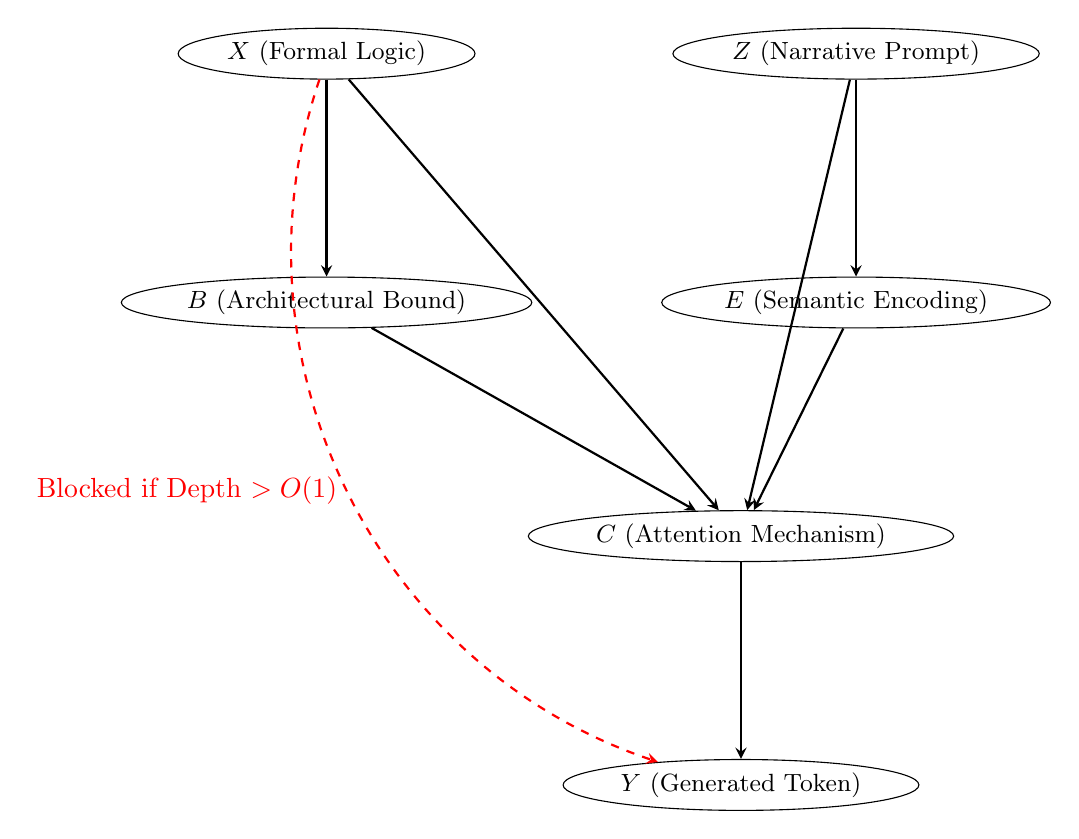
\begin{tikzpicture}[
    node distance=2.5cm and 2.5cm,
    mynode/.style={draw, ellipse, text centered, inner sep=2pt, font=\small},
    myedge/.style={->, thick, >=stealth}
]
\node[mynode] (X) {$X$ (Formal Logic)};
\node[mynode] (Z) [right=of X] {$Z$ (Narrative Prompt)};
\node[mynode] (B) [below=of X] {$B$ (Architectural Bound)};
\node[mynode] (E) [below=of Z] {$E$ (Semantic Encoding)};
\node[mynode] (C) [below right=of B, xshift=-1cm] {$C$ (Attention Mechanism)};
\node[mynode] (Y) [below=of C] {$Y$ (Generated Token)};

\draw[myedge] (X) -- (B);
\draw[myedge] (Z) -- (E);
\draw[myedge] (B) -- (C);
\draw[myedge] (E) -- (C);
\draw[myedge] (X) -- (C);
\draw[myedge] (Z) -- (C);
\draw[myedge] (C) -- (Y);

\draw[myedge, dashed, color=red] (X) to[bend right=45] node[midway, left] {Blocked if Depth $> O(1)$} (Y);
\end{tikzpicture}
\end{center}

\section{The Mechanics of Semantic Gravity}

If the required computational depth of $X$ is within the bound $B$, the logical path $X \to Y$ remains active, and the model achieves perfect accuracy (e.g., depth 1 boolean evaluation).

However, as demonstrated by the Permutation Tracking Limit and the Bounded-Depth Frontier, when the problem depth exceeds $O(1)$, the path $X \to Y$ is structurally severed.

Because $Y$ must still be generated, the causal flow routes entirely through the collider $C$ (the Attention Mechanism). The Attention Mechanism mixes whatever constraints it can parse from $X$ with the overwhelming semantic weight of $E$ (activated by $Z$).

\section{Conclusion}

"Semantic Gravity" ($\Delta_{13}$) is exactly the measure of the path $Z \to E \to C \to Y$.

It is not an "injection" of physical laws across independent boards (Mechanism C), because $C$ operates purely locally within the context window. It is not an "Observer-Dependent Physics," because intervening on $C$ directly alters the effect without changing the observer. It is simply the causal signature of the prompt encoding $E$ taking over the attention heuristic $C$ when the formal logic $X$ is blocked by $B$. The SCM completely explains the empirical data without requiring metaphysical redefinitions.

\end{document}
